% --------------------------------------------------------------------------
% Version 3.0
% This template is available on the sites:
% https://www.overleaf.com/read/rpkkfchcnbsc
% https://www.overleaf.com/latex/templates/itmo-beamer-theme/fpttrgnmqwsb
% https://github.com/AlexZabashta/ITMO-Beamer-theme
% --------------------------------------------------------------------------

% Attention!!!
% This document was created only as an example of using ITMO beamer styling.
% Don't use it as a Latex or beamer tutorial!
% Check out the capabilities of Latex and beamer (at least basic) independently.


\documentclass[aspectratio=169]{beamer}
\usepackage{ITMOtheme}


% Use this package to automatically format references.
% \usepackage[style=mla]{biblatex}
% \addbibresource{references.bib}

% \setbeamertemplate{caption label}{}
\titlegraphic{
\includegraphics[width=0.2\textwidth]{itmo/logo_basic_english_white.pdf}}

% The fields 'title', 'author', 'subject', 'keywords' are used to generate a PDF document.
% It is recommended that you fill them in, even if you are creating your title slide manually.

% use \title[short title]{full title}
\title{Data Wrangling \& Visualization}

%\subtitle[short subtitle]{long subtitle}

\author{Nikita Zagainov, Dmitry Tetkin, Nikita Tsukanov}

%\institute[short institute]{long institute}

\where{Innopolis}
\date{April 2025}


\subject{example}
\keywords{ITMO University, LaTex teamplate, beamer}



\begin{document}


% [plain] - modifier to create a blank slide (without bottom bar).
% Ideal for creating the first (title) and last slide with a polygonal background,
% or for transitional slides between chapters or slides with a table of contents.

% \titlepage - command for automatic generation of title slide content.


% You can use custom title, if you want.
% Or you can you modify the .sty file.


\begin{frame}[plain]
	\itmobackgroundsnakes{
		\vfill
		
\includegraphics[width=0.2\textwidth]{itmo/iu_logo.jpeg}
		\vfill
		\usebeamerfont{title}{  \inserttitle\par}
		\vfill
		UMAP Visualization project
		\vfill
		\insertauthor\par
		\vfill
		\insertplace  \;  \insertdate
	}
\end{frame}


% Avoid making a table of contents in short presentations.
% Transitions between chapters are best done manually.



\begin{frame}{Background: Dimensionality Reduction}
	% add logo at upper-right corner
	\begin{tikzpicture}[remember picture,overlay]
		\node[anchor=north east, xshift=-0.2cm, yshift=-0.2cm]
		at (current page.north east)
		{
\includegraphics[height=1cm]{itmo/kai_logo.png}};
	\end{tikzpicture}

	\begin{itemize}
		\item A powerful tool to compress or simplify data
		\item The most advanced method nowadays - \texttt{UMAP}
		      \footnote{\url{https://arxiv.org/abs/1802.03426}}
	\end{itemize}
	\begin{figure}
		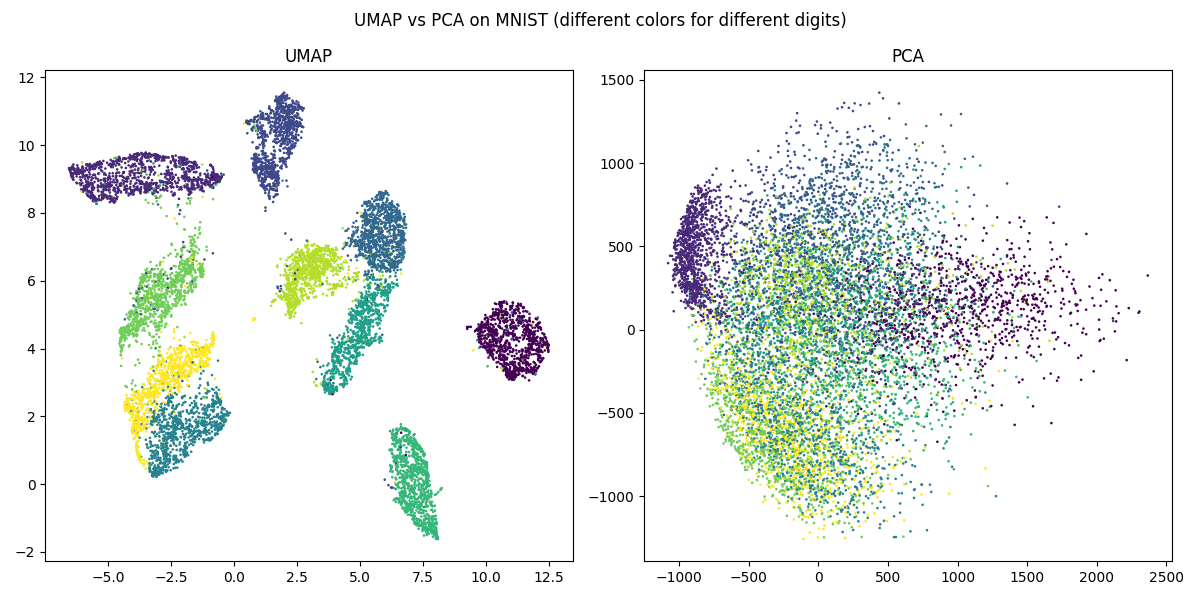
\includegraphics[scale=.3]{fig/pca_vs_umap.png}
		\caption{Different dimensionality reduction algorithms in action}
	\end{figure}
\end{frame}




\begin{frame}
	\frametitle{Project Goal}
	\begin{tikzpicture}[remember picture,overlay]
		\node[anchor=north east, xshift=-0.2cm, yshift=-0.2cm]
		at (current page.north east)
		{
\includegraphics[height=1cm]{itmo/kai_logo.png}};
	\end{tikzpicture}

	\begin{itemize}
		\item To build a web application capable of providing
		      a useful visualization of given high-dimensional dataset
		      in \texttt{.csv} format
		\item To show the process of \texttt{UMAP} algorithm fitting
		      to provided dataset
		\item To provide interactive tools to for exploration of
		      low-dimensional representation of the dataset
	\end{itemize}

\end{frame}



\begin{frame}
	\frametitle{How it works}
	\begin{tikzpicture}[remember picture,overlay]
		\node[anchor=north east, xshift=-0.2cm, yshift=-0.2cm]
		at (current page.north east)
		{
\includegraphics[height=1cm]{itmo/kai_logo.png}};
	\end{tikzpicture}

	\begin{block}{Data preprocessing}
		We created a pipeline to preprocess the data
		and prepare it for visualization. This step is crucial
		as most of the datasets may contain non-numerical features,
		missing values, etc.
	\end{block}

	\begin{block}{UMAP fitting}
		We apply modified version of original \texttt{UMAP} algorithm
		\footnote{\url{https://github.com/lmcinnes/umap}}
		to the preprocessed data to get low-dimensional representation
		of the dataset for 100 consecutive iterations.
	\end{block}

	\begin{block}{Visualization app}
		We use \texttt{FastAPI} framework to deliver embeddings to the
		frontend application, where \texttt{Plotly} library is used to
		visualize the data.
	\end{block}
\end{frame}


\begin{frame}
	\frametitle{Demo}
	\begin{tikzpicture}[remember picture,overlay]
		\node[anchor=north east, xshift=-0.2cm, yshift=-0.2cm]
		at (current page.north east)
		{
\includegraphics[height=1cm]{itmo/kai_logo.png}};
	\end{tikzpicture}

	\begin{figure}
		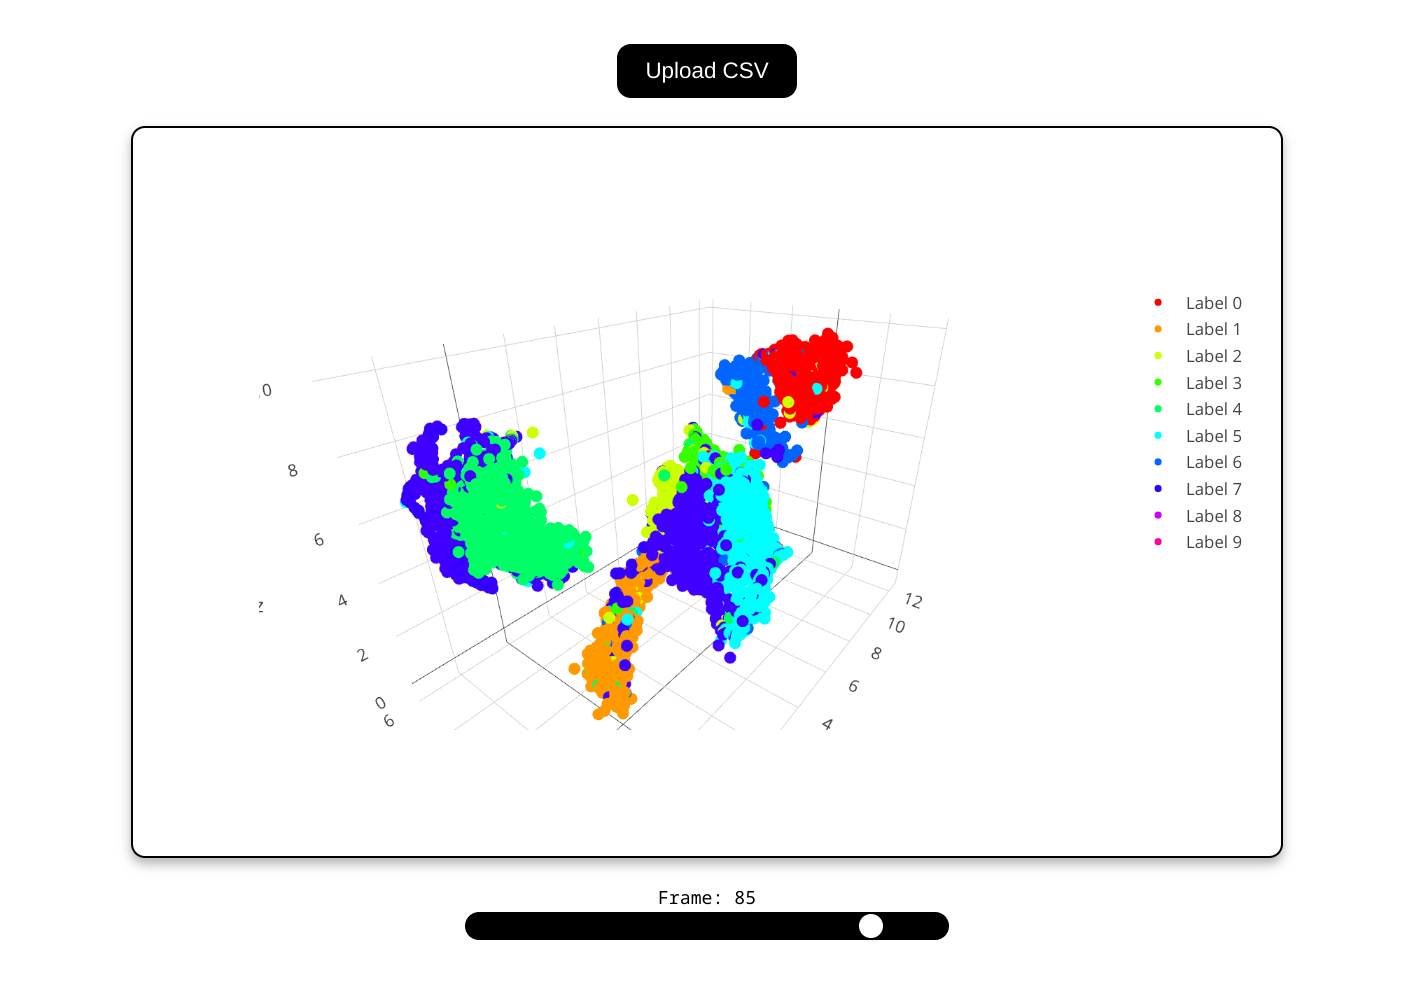
\includegraphics[scale=.23]{fig/demo.png}
		\caption{Demo of the web application}
	\end{figure}

\end{frame}

\begin{frame}
	\frametitle{Useful links}
	\begin{tikzpicture}[remember picture,overlay]
		\node[anchor=center, at=(current page.center), inner sep=0, opacity=0.2]
		{
\includegraphics[width=\paperwidth,height=\paperheight]{itmo/final_slide.png}};
	\end{tikzpicture}

	\begin{columns}[c]
		\column{.45\textwidth}{
			\begin{figure}
				\caption{Follow us on social media!}
				
\includegraphics[width=0.4\paperwidth,height=0.4\paperheight,keepaspectratio]{fig/channel.png}
			\end{figure}
		}

		\column{.45\textwidth}{
			\begin{figure}
				\caption{Project repository}
				
\includegraphics[width=0.4\paperwidth,height=0.4\paperheight,keepaspectratio]{fig/repo.png}
			\end{figure}
		}

	\end{columns}
\end{frame}


\begin{frame}[plain]
	\itmobackgroundsnakes{
		\vfill
		\Huge{Thank you for your attention!}
		\vfill
		
\includegraphics[width=0.4\textwidth]{itmo/slogan.pdf}
	}
\end{frame}


\end{document}
